\chapter{Theoretical Foundation}
\section{X-ray Diffraction}
\begin{figure}[ht]
  \centering
  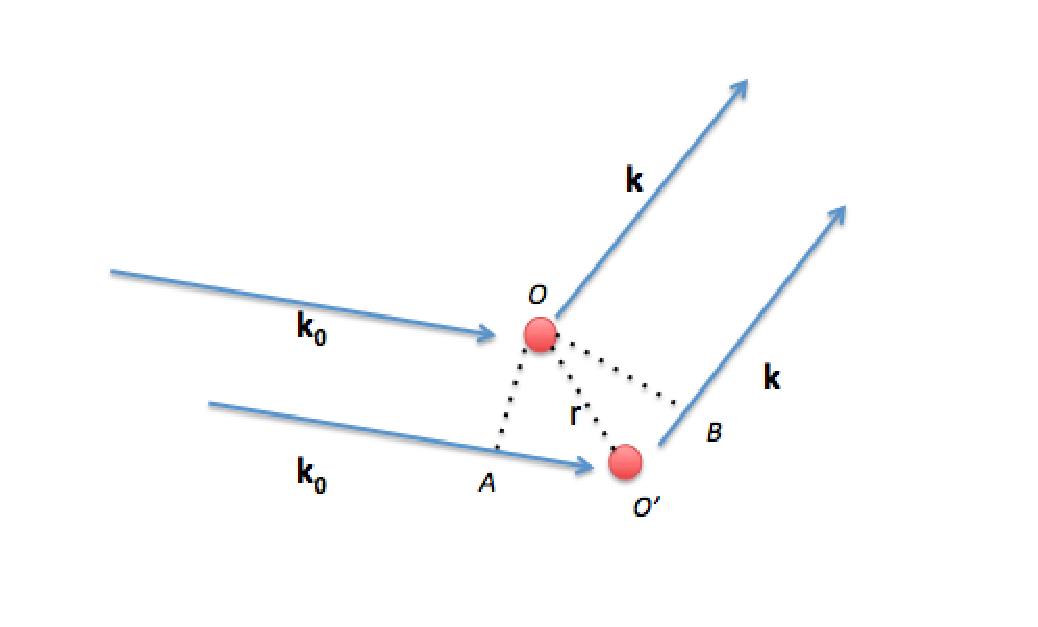
\includegraphics[width=.8\textwidth]{xraydiff}
\caption{Diagram of X-ray diffraction}
\label{fig:xraydiff}
\end{figure}
The diagram in Figure \ref{fig:xraydiff} shows the relation between the incoming waves, the scattered waves and the phase difference. The incoming wave that has wave vector $\vec{k_{0}}$ hits two electrons and they are scattered with the direction of $\vec{k}$. The scattered waves are parallel each other under approximation the observer is very far.

Because the scattered waves are scattered at different positions, the scattered waves will have a phase difference. Another way to see this, the phase difference arise because each scattered waves travel a different length. From figure 1, the bottom wave travels longer than the top wave so that there is a difference in path length.
From figure \ref{fig:xraydiff}, the difference in path length is
\begin{equation}
\mbox{Path difference}=\mbox{AO'}+\mbox{O'B}.
\end{equation}
AO' is projection of $\vec{r}$ along $\vec{k}_{0}$ and has length $\vec{r} \cdot \vec{k}_{0} $. On the other hand, O'B is negative projection of $\vec{r}$ along $\vec{k}$ and has length of $\vec{-r}\cdot \vec{k}$. The total path difference is $\vec{r} \cdot (\vec{k_{0}}-\vec{k})$ or $\vec{r} \cdot \vec{q}$ where $\vec{q}$ is $(\vec{k_{0}}-\vec{k})$ . The total phase difference become $\exp(2 \pi \vec{r} \cdot \vec{q})$.

The diffraction multiplies the amplitude of the scattered wave by a phase factor $\exp(2 \pi \vec{r} \cdot \vec{q})$. If there are many electrons with density $\rho(\vec{r})$ then the effect at particular point $\vec{q}$  will sum to
\begin{eqnarray}
A(\vec{q})=\int \rho(\vec{r}) \exp(2 \pi i \vec{q} \cdot \vec{r}) d \vec{r}.
\label{eq:ftransform}
\end{eqnarray}
So the structure factor appears as a Fourier transform of the electron density. The diffraction experiments only measure the square of absolute value of $A(\vec{q})$, which shows up as the intensity corresponding to $\vec{q}$. Mathematically, the intensity can be written as
\begin{eqnarray}
I(\vec{q})=|A(\vec{q})|^2. 
\label{intensquare}
\end{eqnarray}

There is a more convenient way to calculate a structure factor of the molecule rather than perform Fourier transform of its full electron density. The structure of the molecule can be decomposed into its individual atoms. As already known, there are many the same type of atoms inside the molecule but they differ in positions only. By knowing the Fourier transform of a single type of atom, it leads us to have easier computation because the total structure factor is a sum over all contribution of the Fourier transform of atoms in all position. Thus, calculating the Fourier transform of a single atom enables one to perform easier simulations to calculate structure factors.

The Fourier transform of a single atom is called atomic form factor. Based on a work done by Don Cromer and Mann \cite{CromerMann}, the Hartree-Fock approximation can be used to obtain empirical parameters to approximate atomic form factors. The way they determined the parameters was by fitting 9 parameters in a Gaussian function to a normalized scattering curves. Currently, those parameters are readily available from the international table of crystallography \cite{tablecryst} and the Gaussian function is shown in equation \ref{eq:cromcoef}. 

\begin{center}
  \begin{tabular}{| c | c | c | c | c | c | c | c | c | c | }
    \hline
    atom & $a_1$ & $a_2$ & $a_3$ & $a_4$ & $b_1 $& $b_2$ &$b_3$&$b_4$&$c$ \\ \hline
    C & 2.31 & 1.02 & 1.589 & 0.865 & 20.84 & 10.21 & 0.569 & 51.65 &0.216 \\ \hline
    N & 12.213 & 3.132 & 2.013 & 1.166 & 0.006 & 9.893 & 28.997 & 0.583 &-11.529 \\ \hline
    O & 3.049 & 2.287 & 1.546 & 0.867 & 13.277 & 5.701 & 0.324 & 32.909 & 0.251 \\ \hline
S & 7.070 & 5.340 & 2.236 & 1.512 & 1.366 & 19.828 & 0.092 & 55.228 & -0.159 \\ \hline
  \end{tabular}
\captionof{table}{Table of Cromer-Mann coefficients}\label{tab:ccMco}
\end{center}
\begin{figure}[ht]
  \centering
  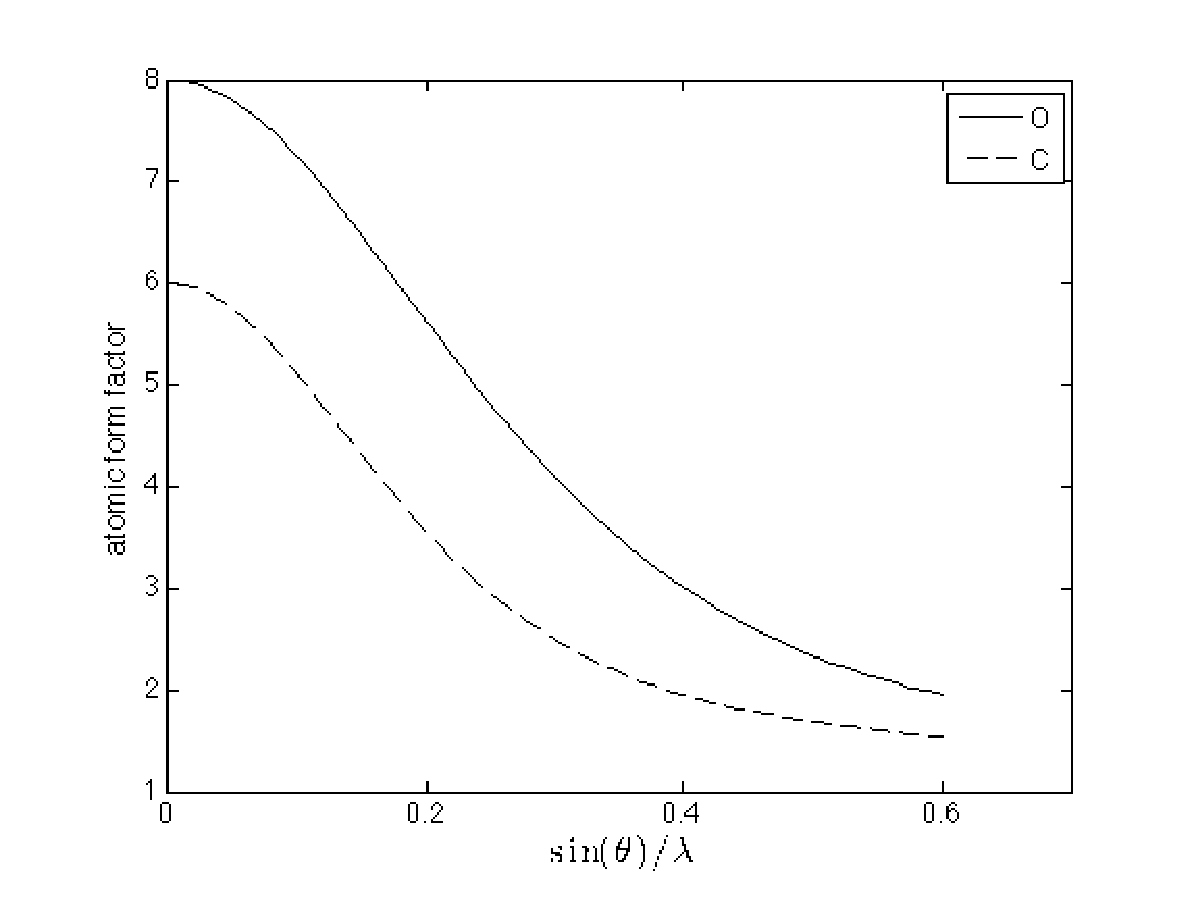
\includegraphics[width=.8\textwidth]{atomicff}
\caption{Plot of atomic form vector for carbon and oxygen}
\label{fig:atomicff}
\end{figure}
The parameters for different type of atoms are listed in table \ref{tab:ccMco}. There are 9 parameters for each atom and the table shows only entries for carbon, oxygen, nitrogen, and sulfur. After knowing all 9 parameters, the atomic form factor can be calculated using Gaussian function:
\begin{equation}
f(\sin(\theta)/\lambda)= \sum_{i=1}^{4} a_{i} \exp(-b_{i}(\sin(\theta)/\lambda)^2)+c. 
\label{eq:cromcoef}
\end{equation}
 A plot of the atomic form for carbon and oxygen is shown in figure \ref{fig:atomicff}. It is shown in the plot that the value of atomic form factor goes to their atomic number when $\sin(\theta)/\lambda$ close to zero.

The structure factor can be calculated in a simpler way if the approximation of atomic form factor is used. Because the atomic form factor is calculated once, the calculation of the structure factor is done faster for all atoms. Finally, the expression for the structure factor in terms of the atomic form factors is described as
\begin{equation}
A(\vec{q})=\sum_{i} f_{i}(q) \exp(2 \pi \vec{q} \cdot \vec{r_i}). 
\label{eq:strfac}
\end{equation}

The equation \ref{eq:strfac} will be used to simulate structure factors for a molecule. As long as a molecule is listed as a collection of atoms in different positions, then equation \ref{eq:strfac} can be used to simulate the structure factor. Some structures of molecules have been solved using methods of crystallography and their structures are available in the protein data bank (pdb). The pdb file describes a molecule as a list of atom type as well as their positions. Having said that, one can simulate a structure factor by using equation \ref{eq:strfac} where the entry is from the pdb file.

\begin{figure}[ht]
  \centering
  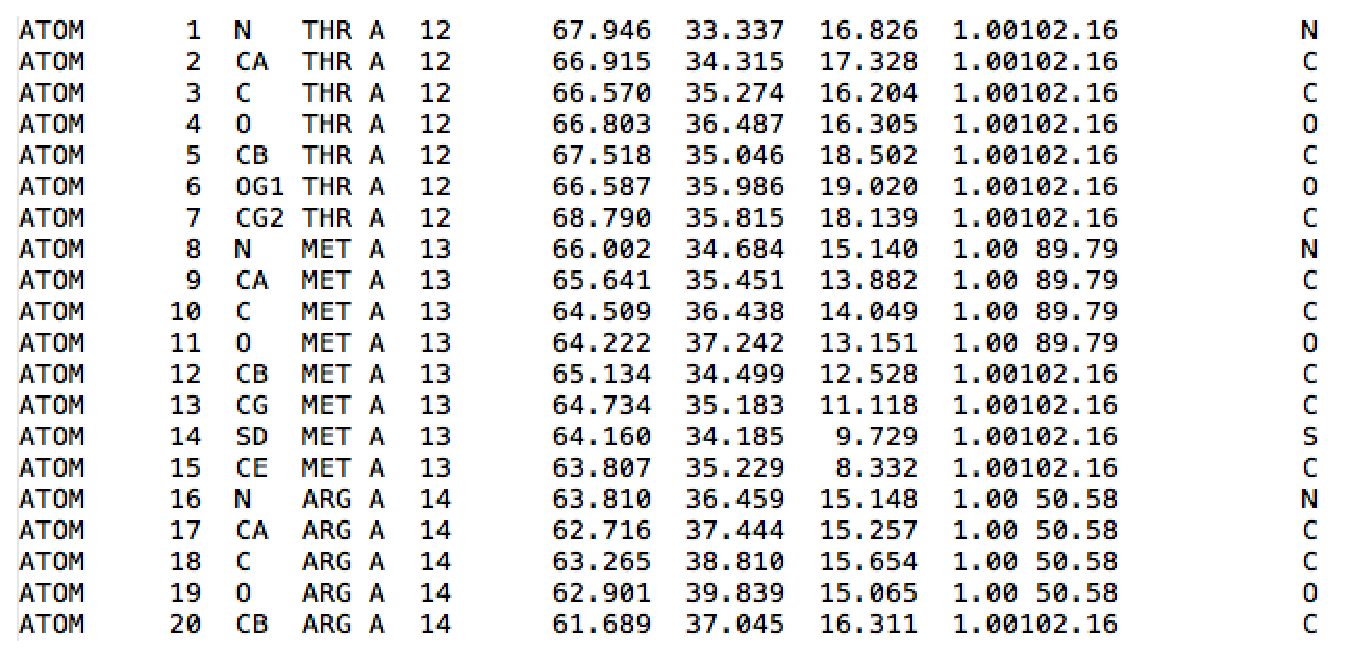
\includegraphics[width=.8\textwidth]{pdbshot}
\caption{Example of data from protein data bank in pdb format}
\label{fig:pdbshot}
\end{figure}

Figure \ref{fig:pdbshot} is a snapshot of a part of the pdb file. In order to read the information from pdb file, one requires to understande thoroughly the format and the convention of the file. First, the pdb file has row entries where each row is a single atom in particular position together with additional information. It consists of multiple columns where each column has particular information. In total, there are 27 columns and all data is in a text file in ASCII format. 

For the purpose of simulating the structure factors, only atom types and their positions are needed. Thus, there are four pieces of information needed, namely atom type, position-x, position-y, and position-z. The atom type is shown between columns 13 to 16. The position-x is shown between columns 31-38. The position-x is shown between columns 39-46. The position-x is shown between columns 47-54. With the information above, the structure factor can be simulated using equation \ref{eq:strfac} with the source of a pdb file. Full explanation about the format of pdb file is given in appendix \ref{ch:pdb}

\section{Angular Correlation} \label{sec:angcor}
\begin{figure}[ht]
  \centering
  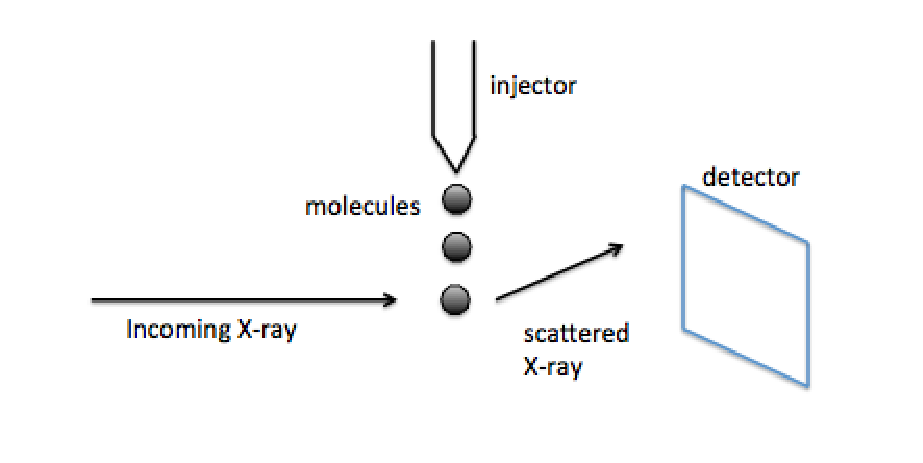
\includegraphics[width=.8\textwidth]{schemadifdes2}
\caption{Diagram of single particle diffraction experiment}
\label{fig:spiexp}
\end{figure}
A single particle diffraction experiment is an experiment that diffracts individual biomolecules using high intensity X-rays without crystallization. Figure \ref{fig:spiexp} shows the schematic design of the experiment.  The incoming X-ray produced in LCLS has high enough intensity so that detector can capture the scattered waves. The injector is capable to stream the molecules in tiny diameter so that there is chance an X-ray will hit a single molecule. 

The information obtainable from this setup is the diffraction patterns of the molecules. However, there is missing information from the setup, namely the information about the orientations of the molecules. Each diffraction pattern recorded by detector is very noisy therefore can't be used for information about the orientation of the molecules. It is important to note that the detector is able to record many millions of diffraction patterns. Although the information about the orientations is lost, it is still possible to get the information about the structure of the molecule by averaging many diffraction patterns. The next section explains the theory to reconstruct the structure of the molecules by averaging many random orientations of the diffraction patterns.  

\begin{figure}[ht]
  \centering
  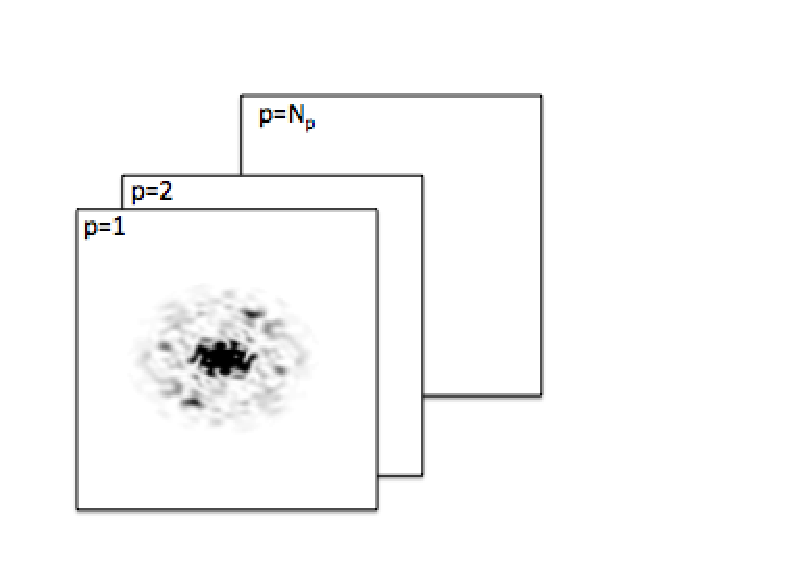
\includegraphics[width=.8\textwidth]{colldp}
\caption{Collection of random angle diffraction patterns}
\label{fig:colldp}
\end{figure}
Figure \ref{fig:colldp} illustrates typical outputs of a diffract and destroy experiment. The output consists of a collection of the diffraction patterns in random orientations. In order to remove the angular dependence, we need to take average over all diffraction patterns. Because the structure of molecule cannot be obtained by only taking average of a point in the diffraction patterns as all point average to the same for random molecules orientations, two points averaging is done to obtain more information about the structure of molecules. The final goal is to derive an angle independent quantity, which has information about the structure, by correlating two points in the diffraction patterns and summing over all diffraction patterns.
\begin{figure}[ht]
  \centering
  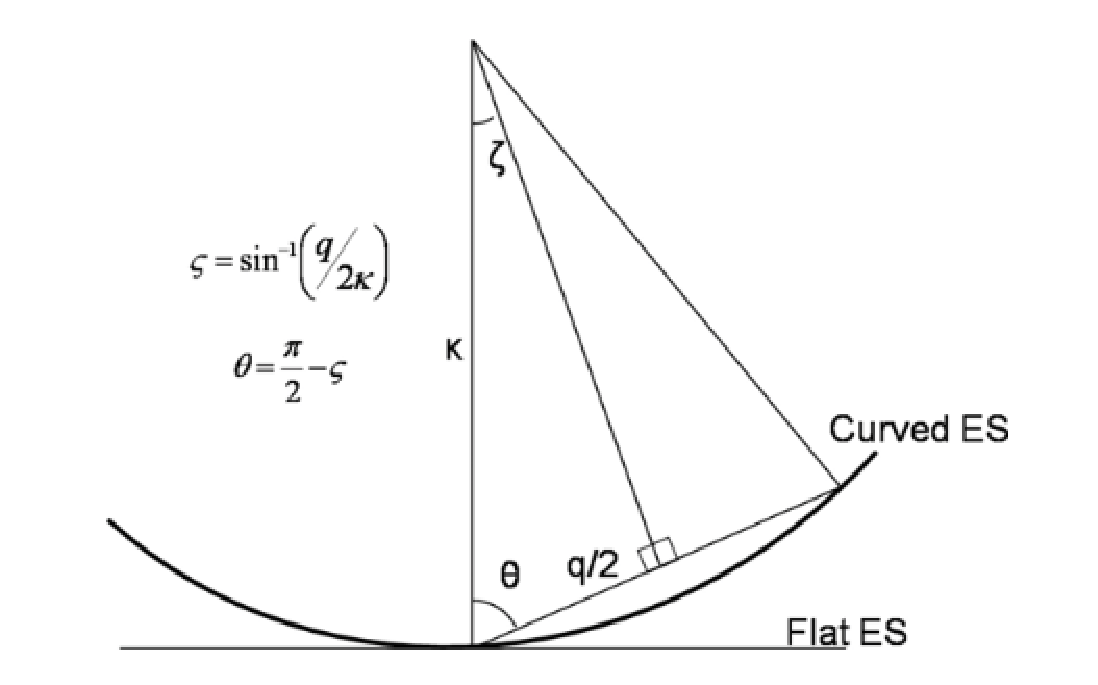
\includegraphics[width=.7\textwidth]{ewsphe}
\caption{Relation between reciprocal radial distance $q$ and angle $\theta$ in an Ewald sphere \cite{saldin2009} }
\label{fig:ewrelation}
\end{figure}

Before going into the derivation of correlations, it is important to derive relation between the intensity and the diffraction pattern. Figure \ref{fig:ewrelation} is a section through the Ewald sphere and a single diffraction pattern samples 3D reciprocal space in Ewald sphere. Consequently, one can derive the relation between the polar angle $\theta$ and the distance $q$, namely 
\begin{eqnarray}
\theta(q) = \frac{\pi}{2} - \sin ^{-1}(\frac{q}{2 \kappa})
\label{eq:thetarelationq}
\end{eqnarray}
as illustrated in figure \ref{fig:ewrelation}.

The curvature of Ewald sphere for arbitrary X-ray wave number $\kappa$ is taken into account correctly by expressing $\theta$ in terms of $q$ and $\kappa$. By substituting $\theta$ in equation \ref{eq:thetarelationq}, any point in a diffraction pattern can be specified by its $q$ and $\phi$ as illustrated in figure \ref{fig:polarcor}. Another step is by taking Z-axis as the direction antiparallel to the incident wave then the measured intensity in a diffraction pattern can be expressed as
\begin{eqnarray}
I_{Z}(q,\phi)=\sum_{lm} I_{lm} Y_{lm}(\theta(q),\phi).
\end{eqnarray} 

Figure \ref{fig:colldp} illustrates that there are many diffraction patterns and index $p$ corresponds to the diffraction patterns with different molecular orientations. The orientation can be seen as a rotation of frame of reference because a rotation of the molecule is equivalent to an inverse rotation of its frame of reference. Mathematically, the particular orientation can be expressed by applying rotation operator to its original basis function. Specifically, the rotation operator is matrix $D_{lm}$ because we chose spherical harmonics as basis function of intensity. Consequently, the new diffraction pattern in rotated frame of reference is  
\begin{eqnarray}
I^{(p)}(q,\phi)=\sum_{lmm'}I_{lm}(q) D^{(p)}_{lmm'}(\alpha,\beta,\gamma) Y_{lm'}(\theta(q),\phi).
\label{Idiffrot}
\end{eqnarray}

\begin{figure}[ht]
  \centering
  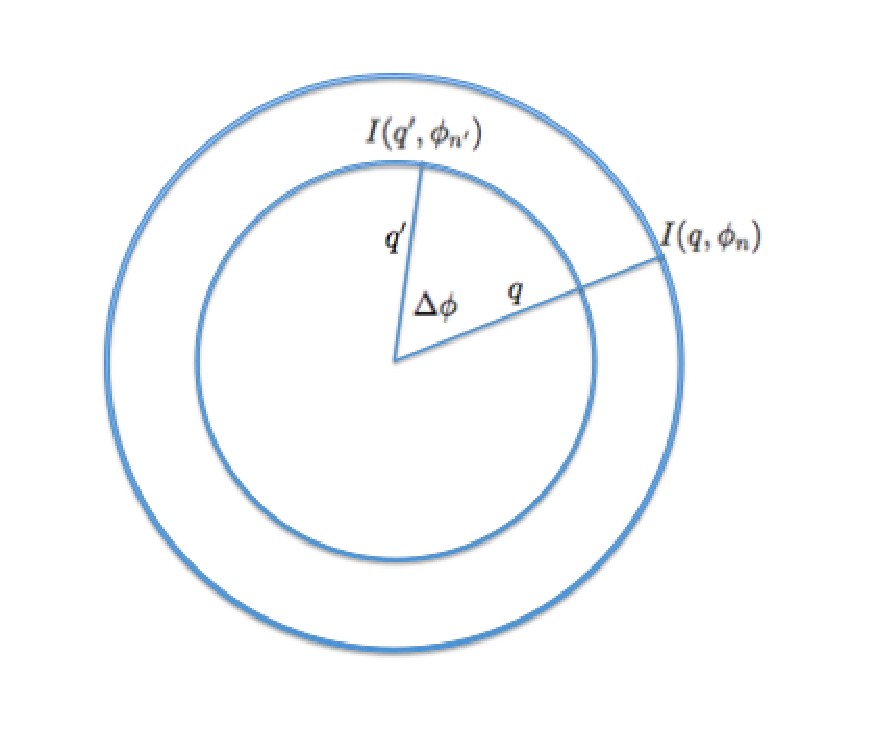
\includegraphics[width=.8\textwidth]{polarcor}
\caption{Two points correlation in a diffraction pattern}
\label{fig:polarcor}
\end{figure}

The first step in using this method is to calculate angular cross correlations on each diffraction pattern  in polar coordinates. Polar coordinates are natural for this problem since the particles differ mainly in their orientations (They may also differ in position, but this does not affect the diffraction pattern intensities that are insensitive to the particle phases).

As illustrated in figure \ref{fig:polarcor}, we can pick any two points in the polar diffraction pattern by specifying the coordinate $q$ and angle $\phi$.  The next step is to correlate every point in rings $q$ and $q'$ by keeping the same angular distance  $\phi$ and $\phi'$. Angular pair correlations are defined by
\begin{eqnarray}
C_{2}(q,q',\phi,\phi') &=& \frac{1}{N_{p}} \sum_{p} I^{(p)}(q,\phi) I^{(p)}(q',\phi') 
\label{eq:crosscor}
\end{eqnarray}
where $p$ is the index of the diffraction patterns and $N_p$ is the total number of diffraction pattterns as illustrated in figure \ref{fig:colldp}.

Equation \ref{eq:crosscor} can be expressed in terms of summation of points in diffraction patterns rotated by matrix $D^{(p)}_{lm}$. By substituting equation \ref{Idiffrot} into equation \ref{eq:crosscor}, the $C_{2}$ become
\begin{align}
\begin{split}
C_{2}(q,q',\phi,\phi') = \frac{1}{N_{p}} &  \sum_{p} \sum_{lmm'} \sum_{l'm''m'''}I^{*}_{lm}(q) D^{(p)*}_{lmm'} Y^{*}_{lm'}(\theta(q),\phi) \\
&\times I_{l'm''}(q) D^{(p)}_{l'm''m'''} Y_{l'm'''}(\theta'(q'),\phi') 
\label{eq:crossDangle}
\end{split}
\end{align}

The Wigner $D$-matrices are representation of the full rotation group. A set of the Euler angles specify the rotation of matrix $D$. Due to the randomness of the orientations of the diffraction patterns, the larger the number of diffraction patterns the most likely the angles will occupy the entire space. Under assumption that the set of random angles will converge into all uniform rotational angles then equation \ref{eq:crossDangle} can be simplified. The relation that is used to simplify the equation is called the orthogonality theorem, which mathematically expressed as
\begin{eqnarray}
\frac{1}{N} \sum_{(p)} D^{(p)*}_{lmm'} D^{(p)}_{l'm''m'''}=\frac{1}{2l+1} \delta_{ll'} \delta_{mm''} \delta_{m'm'''}.
\label{eq:orthotheorem}
\end{eqnarray}

By summing over $p$ in equation \ref{eq:crossDangle}, making use of the great orthogonality relation in equation \ref{eq:orthotheorem}, and then summing over $l'$, $m''$, and $m'''$ will transform equation \ref{eq:crossDangle} into 
\begin{eqnarray}
C_{2}(q,q',\phi,\phi') = \sum_{l} F_{l}(q,q';\phi,\phi') B_{l}(q,q')
\label{C2definition}
\end{eqnarray}
where
\begin{eqnarray}
F_{l}(q,q';\phi \phi') &=& \frac{1}{2l+1} \sum_{m} Y^{*}_{lm}(\theta(q),\phi) Y_{lm}(\theta'(q'),\phi') \\
&=&\frac{1}{4} P_{l} [\cos \theta (q) \cos \theta (q') + \sin \theta(q) \sin \theta(q') \cos(\phi-\phi') ]
\label{eq:FP}
\end{eqnarray}
where $P_{l}$ is a Legendre polynomial of order l, and
\begin{eqnarray}
B_{l}(q,q') &=& \sum_{m} I_{lm}(q) I_{lm}^{*}(q').
\label{eq:theB}
\end{eqnarray}
The left hand side of equation \ref{C2definition} is obtainable from experiment. The first term of right hand side of equation \ref{C2definition} can be calculated mathematically. Consequently, the quantity $B_{l}$ can be obtained from experiment and it can be used to get the information about the structure of the molecule.

The calculation to extract $B_{l}$ from equation \ref{C2definition} is matrix inversion. For each pair $q$ and $q'$, equation \ref{C2definition}  may be written as the matrix equation
\begin{eqnarray}
C_{2(\phi\phi')}=\sum_{l} F_{\phi\phi',l}B_{l}.
\end{eqnarray}
All elementes of matrix $F$ are real number. Thus, the above equation can be inverted to get real coefficients $B_{l}$ where
\begin{eqnarray}
B_{l}=\sum_{\phi \phi'} {F^{-1}}_{l,\phi \phi'} C_{2(\phi \phi')}.
\label{eq:Binvert}
\end{eqnarray}

The above equation can be used to calculate \Blq after $C_{2}$ is obtained. 
The information about the structure of the molecules is contained in \Blq because \Blq contain information about $I_{lm}(q)$ where $I_{lm}(q)$ are spherical harmonic expansion of a diffraction volume. Thus, the information about the structure of molecules can be obtained by calculating \Blq from a set of random angle diffraction patterns.

The spherical harmonics are used to expand the diffraction volume because it can construct any function in a 2D surface. In 3D case, a molecule is free to rotate in any two angles, namely azimuthal and polar angle. However, in 2D case only rotation with respect to single axis is allowed. Thus, a basis functions with single rotation is simpler to be used than spherical harmonics. 

Beside spherical harmonics, circular harmonics can be used to expand the intensity as long as the random angles only have a single axis. The expression of the diffraction patterns in terms of circular harmonic expansion can be written 
\begin{eqnarray}
I(q,\phi)= \sum_{m} I_{m}(q) \exp(im\phi).
\label{eq:Imq}
\end{eqnarray}
This is derived similarly as before, by substituting equation \ref{eq:Imq} into equation \ref{eq:crosscor} and performing the average over all diffraction patterns,the new $C_{2}$ with respect to circular harmonics become
\begin{eqnarray}
C_{2}(q,q';\phi \phi')=\sum_{m} I^{*}_{m}(q) I_{m}(q') \exp(im(\phi-\phi'))
\label{eq:c2Imq}
\end{eqnarray}
where \Imq is the circular harmonic expansion coefficients of the diffracted intensity of a single particle. The right hand side of equation \ref{eq:c2Imq} 
is an exponential function. By multiplying both side with its inverse and integrating over all angles, it will remove the dependence of the exponential function in the right hand side of the equation. Thus, a new quantity can be obtained, namely
\begin{eqnarray}
B_{m}(q,q')&=&\int C_{2}(q,q',\Delta \phi) \exp(-i m \Delta \phi) d\Delta\phi= I_{m}(q)^{*} I_{m}(q') \\
\label{eq:Bmqdef}
\end{eqnarray}

The information about the structure is contained in the quantity $I_{m}(q)$. The magnitude of $I_{m}(q)$ is directly accessible by taking square root of the diagonal values of \Bmq. For that reason, the phase of $I_{m}(q)$ is the only missing information to fully determine $I_{m}(q)$ from \Bmq. After $I_{m}(q)$ is determined, the reconstruction of the intensity distribution of a single molecule can be found from equation \ref{eq:Imq}. 

Now after deriving \Blq and \Bmq, there is another quantity that is very important for reconstruction of structure of the molecule, namely two point angular triple correlations. Mathematically, it is defined by \cite{kam1978}
\begin{eqnarray}
C_{3}(q,q',\phi,\phi') &=& \frac{1}{N_{p}} \sum_{p} I_{p}^{2}(q,\phi) I_{p}(q',\phi') 
\label{eq:crosstripcor}
\end{eqnarray}

Similar derivation as before, the expansion coefficients in equation \ref{Idiffrot} are substituted into equation \ref{eq:crosstripcor}. The result of substitution is
\begin{align}
\begin{split}
C_{3}(q,q',\phi,\phi') &= \frac{1}{N_{p}} \sum_{p} \sum_{l_{1},l_{2},l_{3}} \sum_{m_{1},m_{2},m_{3}} \sum_{m'_{1},m'_{2},m'_{3}} \\ 
&\times I_{l_{1}m_{1}} D_{l_{1}m_{1}m'_{1}}(\omega) Y_{l_{1}m'_{1}}(\theta,\phi) \\ 
&\times I_{l_{2}m_{2}} D_{l_{2}m_{2}m'_{2}}(\omega) Y_{l_{2}m'_{2}}(\theta,\phi) \\ 
&\times I^{*}_{l_{3}m_{3}} D^{*}_{l_{3}m_{3}m'_{3}}(\omega') Y^{*}_{l_{3}m'_{3}}(\theta,\phi' ). \\ 
\label{eq:c3subs}
\end{split}
\end{align}

To simplify the above equation, these relations are substituted into the above equation:
\begin{align}
\label{eq:triprel1}
\begin{split}
D_{l_{1}m_{1}m'_{1}}(\omega) D_{l_{2}m_{2}m'_{2}}(\omega)&= \sum^{l_1+l_2}_{L=|l_1-l_2|} \sum_{(M,M')=-L}^{L}(2L+1)(-1)^{M-M'}  \\ 
&\times\left( \begin{array}{ccc}
l_1 & l_2 & L \\
m_1 & m_2 & -M  \end{array} \right)  \\ 
&\times\left( \begin{array}{ccc}
l_1 & l_2 & L \\
m'_1 & m'_2 & -M'  \end{array} \right) D_{LMM'}(\omega), 
\end{split}
\end{align}

\begin{align}
\label{eq:triprel2}
\begin{split}
Y_{l_1 m'_1}(\Omega)Y_{l_2 m'_2}(\Omega) &= \sum_{\lambda=|l_1-l_2|}^{l_1+l_2} \sum_{\mu=\lambda}^{+\lambda} \left[\frac{(2l_1+1)(2l_2+1)(2l_1+1)}{4 \pi}\right]^{1/2} \\
&\times \left( \begin{array}{ccc}
l_1 & l_2 & \lambda \\
0 & 0 & 0  \end{array} \right)  \\ 
&\times \left( \begin{array}{ccc}
l_1 & l_2 & \lambda \\
m_1' & m_2' & \mu  \end{array} \right) Y_{\lambda\mu}(\Omega), \\  
\end{split}
\end{align}

\begin{align}
\sum_{m'_1 m'_2}\left( \begin{array}{ccc}
l_1 & l_2 & \lambda \\
m'_1 & m'_2 & \mu  \end{array} \right) 
\left( \begin{array}{ccc}
l_1 & l_2 & l_3 \\
m'_1 & m'_2 & -m'_3  \end{array} \right) 
=\frac{1}{2l_3+1} \delta_{\lambda l_3}\delta_{\mu m'_3}, 
\label{eq:triprel3}
\end{align}
and
\begin{align}
\sum_{m'3} Y_{lm'_3}(\theta,\phi) Y^{*}_{lm'_3}(\theta,\phi')=\frac{2l+1}{4 \pi} P_{l}(\cos(\phi-\phi')) 
\label{eq:triprel4}
\end{align}
where the quantities represented by the large parentheses are Wigner $3j$ symbols.

After substituting equations \ref{eq:triprel1}, \ref{eq:triprel2}, \ref{eq:triprel3}, and \ref{eq:triprel4} into equation \ref{eq:c3subs}, the equation \ref{eq:c3subs} become
\begin{align}
\begin{split}
C_{3}(q,q',\Delta \phi)&= \sum_{l_1 l_2 l} \sum_{m_1 m_2 m} I_{l_1 m_1}(q) I_{l_2 m_2}(q) I^{*}_{l m}(q') P_{l}(\cos(\Delta \phi)) \\ 
&\times (-1)^{m}(4\pi)^{-\frac{3}{2}} 
\left( \begin{array}{ccc}
l_1 & l_2 & l \\
m_1 & m_2 & -m  \end{array} \right) 
\left( \begin{array}{ccc}
l_1 & l_2 & l \\
0 & 0 & 0  \end{array} \right)  \\ 
&\times \left[(2l_1+1)(2l_2+1)(2l_1+1)\right]^{1/2}.
\end{split}
\label{eq:tripc3}
\end{align}

Additional relation is needed to invert the equation \ref{eq:tripc3}. The relation is orthogonality of the Legendre polynomials, the mathematical expression is
\begin{eqnarray}
\int_{-1}^{1} P_{l}(u) P_{l'}(u) du =\frac{2}{2l+1} \delta_{ll'}. 
\end{eqnarray}
A new quantity $T_{l}(q,q')$ is obtained by applying the orthogonality of the Legendre polynomials into equation \ref{eq:tripc3}. The $T_{l}(q,q')$ can be written as
\begin{align}
\begin{split}
T_{l}(q,q')&=\int C_{3}(q,q',\Delta \phi)  P_{l}(\cos(\Delta \phi)) d(\Delta \phi) \frac{(2 l+1)}{2} 4 \pi \\ 
\label{eq:tripleexp}
\end{split}
\end{align}
or theoretically can be calculated from
\begin{align}
\begin{split}
T_{l}(q,q')&= \sum_{l_1,l_2,m_1,m_2,m} (-1)^m
 \left[\frac{(2l_1+1)(2l_2+1)(2l_1+1)}{4 \pi}\right]^{1/2}
 \left( \begin{array}{ccc}
l_1 & l_2 & l \\
0 & 0 & 0  \end{array} \right) 
 \left( \begin{array}{ccc}
l_1 & l_2 & l \\
m_1 & m_2 & -m  \end{array} \right)  \\ 
&  I_{l_1,m_1}(q) I_{l_2,m_2}(q) I_{l,m}(q).       
\label{eq:triple}
\end{split}
\end{align}

Apart from \Blq, the information about the structure of the molecule can be obtained from $T_{l}(q,q')$ as well. The $C_{3}$ is a quantity that is obtainable from experiment data as described in equation \ref{eq:crosstripcor}. Thus, $T_{l}(q,q')$ can be calculated from experiment data as described in equation \ref{eq:tripleexp}. As a result of that, $T_{l}(q,q')$ can be used to reveal the information about the structure of the molecule because it involves the summation over spherical harmonics expansion of the diffraction volume.
\subsection{Independent Parameters}
As stated before, \Blq is one of the quantities measurable in the experiment. The objective of this method is to obtain the electron density from the \Blq. If the diffraction volume or intensity can be obtained from \Blq then the diffraction volume can be phased using a phasing algorithm to get the electron density. Having said that, it is important to study relationship between \Blq and \Ilm. 

For a given \Blq, \Ilm cannot be determined uniquely. The reason of that is a new \Ilm can be formed by multiplying it by orthogonal matrix. 
\begin{eqnarray}
I_{lm}'(q)=O^{l}_{mm'}I_{lm'}(q)  \\
\mbox{where} \quad O^{l}_{mm'} (O^{l}_{mm'})^{\dagger} =1. 
\label{eq:ilmolm}
\end{eqnarray}
In other words, if a matrix $O^{l}_{mm'}$ is unitary or orthogonal then the value of \Blq is not affected by multiplication of any orthogonal matrix as shown below:
\begin{eqnarray}
B_{l}'(q,q')&=&\sum_{m} I_{lm}'(q) I_{lm}'^{\dagger}(q') \\
B_{l}'(q,q')&=&\sum_{m} I_{lm}(q) O^{l}_{m'm''} (O^{l}_{m'm''})^{\dagger} I_{lm}^{\dagger}(q') \\ \nonumber
B_{l}'(q,q')&=&\sum_{m} I_{lm}(q)  I_{lm}^{\dagger}(q') \\ \nonumber
B_{l}'(q,q')&=&B_{l}(q,q'). \\ \nonumber
\label{eq:Blilmolm}
\end{eqnarray}

For each $l$, there are unitary matrices $O^{l}_{mm'}$ that contribute to the nonuniqueness of \Ilm. The matrices $O^{l}_{mm'}$ have $2l+1$ rows and $2l+1$ columns. The total elements of the particular matrix is $(2l+1)^2$. However, not all elements are independent of each other because the matrix satisfy orthogonality. 

From \cite{tinkham}, an $n \times n$ orthogonal matrix has $\frac{n(n-1)}{2}$ independent elements. Since an $O^{l}_{mm'}$ has $(2l+1)$x$(2l+1)$ elements then the total independent elements for a particular $l$ is $(2l+1)(l)$ elements. 

Given the explanation above, the total elements is
\begin{eqnarray}
\sum_{l=0,2,4,...}^{l_{max}} (2l+1)(l).
\label{eq:indcomp}
\end{eqnarray}

